\textbf{Lưu ý:} đây chỉ là lý thuyết báo cáo tự đề xuất ra cho nên vẫn chưa được kiểm chứng hoàn toàn.

Abstract Meaning Representation (AMR) là một dạng biểu diễn ngữ nghĩa trừu tượng, dùng để mô tả ý nghĩa của câu theo cách ngôn ngữ độc lập\cite{amr-guidelines}. AMR tập trung vào việc biểu diễn cấu trúc ngữ nghĩa của câu dưới dạng đồ thị, trong đó các đỉnh là các khái niệm hoặc thực thể, và các cạnh biểu diễn mối quan hệ giữa các khái niệm này.

AMR nắm bắt được “ai đang làm gì với ai” trong một câu. Mỗi câu được biểu diễn dưới dạng một đồ thị có gốc, có hướng, và không chu trình với các nhãn trên các cạnh (quan hệ) và các lá (khái niệm)\cite{amr-guidelines}.

Giống như một cây phân tích cú pháp, AMR cung cấp một cấu trúc duy nhất có thể duyệt qua mà tính đến tất cả các từ. Nó không phải là một tập hợp các lớp chú thích rời rạc. Không giống như cây phân tích cú pháp, AMR là trừu tượng. Nó có thể biểu diễn nhiều câu ngôn ngữ tự nhiên khác nhau. AMR không chú thích các từ riêng lẻ trong một câu, như một phân tích phụ thuộc\cite{amr-guidelines}.

\begin{figure}[H]
    \centering
    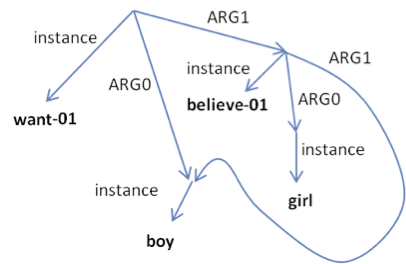
\includegraphics[width=0.7\linewidth]{Images/GDL/amr_ex.png}
    \caption{Ví dụ minh họa về AMR\cite{amr-guidelines}}
    \label{fig:ex_amr}
\end{figure}

Câu AMR trong hình \ref{fig:ex_amr} có nghĩa là: Có một sự kiện mong muốn, trong đó ARG0 (người mong muốn) là một cậu bé, và ARG1 (điều được mong muốn) là một sự kiện tin tưởng. Sự kiện tin tưởng này có ARG0 (người tin tưởng), là một cô gái, và nó có ARG1 (điều được tin tưởng), chính là cậu bé vừa được nhắc đến. Ở đây, cậu bé đóng hai vai trò: (1) là ARG0 của "want-01", và (2) là ARG1 của "believe-01". AMR thể hiện điều này bằng hai cạnh có hướng trỏ đến cùng một nút. (Theo OntoNotes, các giác quan của vị ngữ được đánh dấu bằng hậu tố như -01 và -02, trong khi ARG0, ARG1, v.v., chỉ các vai trò cốt lõi, cụ thể của vị ngữ.)

\begin{figure}[H]
    \centering
    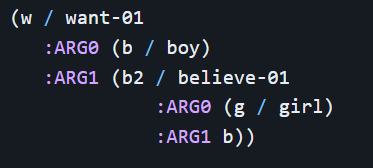
\includegraphics[width=1\linewidth]{Images/GDL/amr_ex_text.png}
    \caption{Biểu diễn AMR dạng text của ví dụ trong hình \ref{fig:ex_amr}}
\end{figure}

Kể từ khi ra đời, AMR đã được áp dụng rộng rãi trong nhiều lĩnh vực xử lý ngôn ngữ tự nhiên. Các ứng dụng phổ biến bao gồm dịch máy, tóm tắt văn bản, trả lời câu hỏi, và phân tích cảm xúc. Sự đa dạng trong ứng dụng này chứng tỏ tính linh hoạt và hữu ích của AMR trong việc nắm bắt và biểu diễn ý nghĩa ngôn ngữ.

Song song với sự phát triển về ứng dụng, nhiều công cụ đã được tạo ra để hỗ trợ việc tự động hóa quá trình tạo và phân tích AMR. Các công cụ này bao gồm các bộ phân tích cú pháp tiên tiến và các mô hình học máy phức tạp, giúp tăng cường khả năng xử lý AMR ở quy mô lớn.

Mặc dù ban đầu AMR được phát triển chủ yếu cho tiếng Anh, nhưng theo thời gian, nó đã được mở rộng để hỗ trợ nhiều ngôn ngữ khác. Điều này đã mở ra cơ hội cho việc áp dụng AMR trong các nhiệm vụ xử lý ngôn ngữ đa ngôn ngữ và liên ngôn ngữ.

Quá trình phát triển của AMR vẫn đang tiếp diễn. Các nhà nghiên cứu liên tục cải tiến và mở rộng khả năng của AMR để xử lý các hiện tượng ngôn ngữ ngày càng phức tạp hơn, đồng thời tăng độ chính xác trong biểu diễn ngữ nghĩa. Những nỗ lực này nhằm đảm bảo rằng AMR vẫn là một công cụ mạnh mẽ và linh hoạt trong lĩnh vực xử lý ngôn ngữ tự nhiên, có khả năng đáp ứng các thách thức mới nổi trong việc hiểu và biểu diễn ngôn ngữ tự nhiên.

Trong lĩnh vực dịch máy, AMR đóng vai trò quan trọng như một biểu diễn trung gian. Bằng cách chuyển đổi văn bản nguồn thành AMR, sau đó từ AMR sang ngôn ngữ đích, các hệ thống dịch có thể nắm bắt được ý nghĩa sâu sắc của văn bản, giúp tạo ra bản dịch chính xác và tự nhiên hơn. Phương pháp này đặc biệt hiệu quả khi xử lý các cặp ngôn ngữ có cấu trúc khác biệt lớn.

AMR cũng được sử dụng rộng rãi trong tác vụ tóm tắt văn bản. Bằng cách biểu diễn nội dung chính của văn bản dưới dạng đồ thị AMR, các hệ thống có thể dễ dàng xác định và trích xuất thông tin quan trọng, từ đó tạo ra các bản tóm tắt ngắn gọn và đầy đủ nội dung.

Trong lĩnh vực trả lời câu hỏi, AMR giúp phân tích cả câu hỏi và các đoạn văn bản tiềm năng chứa câu trả lời. Việc so sánh cấu trúc AMR của câu hỏi và văn bản cho phép hệ thống xác định chính xác thông tin cần thiết để đưa ra câu trả lời phù hợp.

AMR cũng được ứng dụng trong phân tích cảm xúc và khai thác ý kiến. Bằng cách biểu diễn cấu trúc ngữ nghĩa của câu, AMR giúp hệ thống nắm bắt được các sắc thái tinh tế trong cảm xúc và quan điểm được thể hiện, vượt ra ngoài phân tích đơn thuần dựa trên từ khóa.

Trong lĩnh vực sinh văn bản tự động, AMR được sử dụng như một khuôn mẫu ngữ nghĩa. Các hệ thống có thể tạo ra văn bản mạch lạc và có ý nghĩa bằng cách sinh câu từ biểu diễn AMR, đảm bảo rằng nội dung được tạo ra phù hợp với ý định ngữ nghĩa mong muốn.

Ngoài ra, AMR còn được áp dụng trong nhiều lĩnh vực khác như phân tích diễn ngôn, trích xuất quan hệ, và hệ thống đối thoại. Trong mỗi trường hợp, khả năng nắm bắt ý nghĩa sâu sắc của AMR giúp cải thiện hiệu suất và độ chính xác của các hệ thống xử lý ngôn ngữ tự nhiên.

Tiếp theo, báo cáo sẽ đưa ra hai ví dụ về AMR của hai câu đồng nghĩa sau:

- "The scientist who discovered the new element won the Nobel Prize and inspired young researchers around the world."

- "The Nobel Prize was awarded to the scientist who found the new element, and this achievement motivated young researchers globally."

\begin{figure}[H]
    \centering
    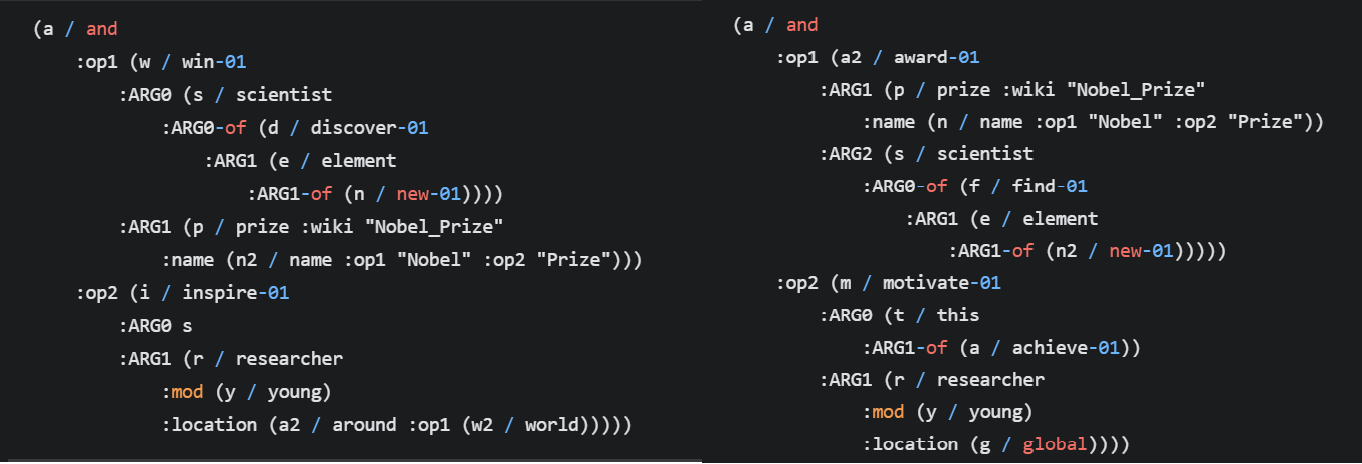
\includegraphics[width=1\linewidth]{Images/GDL/amr_2_sym.png}
    \caption{Biểu diễn AMR của hai câu đồng nghĩa}
    \label{fig:amr_sym}
\end{figure}

Từ hình \ref{fig:amr_sym} có thể thấy rằng cả hai AMR đều thể hiện được hai sự kiện chính: việc một nhà khoa học được trao giải Nobel vì phát hiện ra nguyên tố mới, và việc thành tựu này truyền cảm hứng/thúc đẩy các nhà khoa học trẻ. Bên cạnh đó, các thực thể chính (nhà khoa học, giải Nobel, nguyên tố mới) đều được xác định rõ ràng trong cả hai AMR. Mối quan hệ ngữ nghĩa giữa các thực thể cũng được thể hiện rõ ràng bằng các nhãn vai trò ngữ nghĩa (ARG0, ARG1, ARG0-of, ARG1-of, mod, location).

Tuy nhiên, hai AMR có sự khác biệt về cấu trúc. AMR bên trái sử dụng cấu trúc phức tạp hơn với nhiều mệnh đề con lồng nhau, trong khi AMR bên phải có cấu trúc đơn giản hơn với hai mệnh đề chính được nối với nhau bởi "and".

Sự lựa chọn động từ trung tâm để diễn tả sự kiện được trao giải Nobel cũng khác nhau. AMR bên trái sử dụng động từ "win" (chiến thắng), trong khi AMR bên phải sử dụng "award" (trao thưởng). Việc lựa chọn động từ này ảnh hưởng đến cấu trúc và cách thức thể hiện vai trò ngữ nghĩa trong mỗi AMR.

Phạm vi ảnh hưởng của sự kiện "truyền cảm hứng/thúc đẩy" cũng được thể hiện khác nhau. Trong khi AMR bên trái thể hiện sự kiện "truyền cảm hứng" có phạm vi ảnh hưởng là "các nhà khoa học trẻ trên toàn thế giới", thì AMR bên phải lại thể hiện sự kiện "thúc đẩy" có phạm vi ảnh hưởng là "toàn cầu" (không chỉ giới hạn ở các nhà khoa học trẻ).

Cuối cùng, vị trí của thông tin về phạm vi ảnh hưởng cũng khác nhau. AMR bên trái đặt thông tin về phạm vi ảnh hưởng ("around the world") ở cuối câu, trong khi AMR bên phải đặt thông tin này ("globally") gần với động từ "motivate".

Như vậy, có thể thấy rằng với hai câu khác nhau nhưng cùng ý nghĩa thì khi ta chuyển sang AMR thì sẽ cho ta hai đồ thị AMR khác nhau. Hệ quả, nên tồn tại một quan hệ xác suất giữa hai đồ thị AMR trong một văn cảnh nào đấy. 

Do đó, không gian các đồ thị AMR có thể đưa ra ý tưởng về một cấu trúc mới. Hãy xem xét khái niệm tương đương (equivalence) như một tập hợp các mũi tên: có thể đảo ngược và có thể kết hợp (composable). Điều này dẫn đến việc hình thành một cấu trúc groupoid (groupoid structure). Tuy nhiên, ngoài cấu trúc groupoid, còn có nhiều cấu trúc khác có thể áp dụng. Ví dụ, ta có thể định nghĩa một hàm trên đồ thị AMR để mô tả tần suất sử dụng các phần tử trong đồ thị.

\begin{figure}[H]
    \centering
    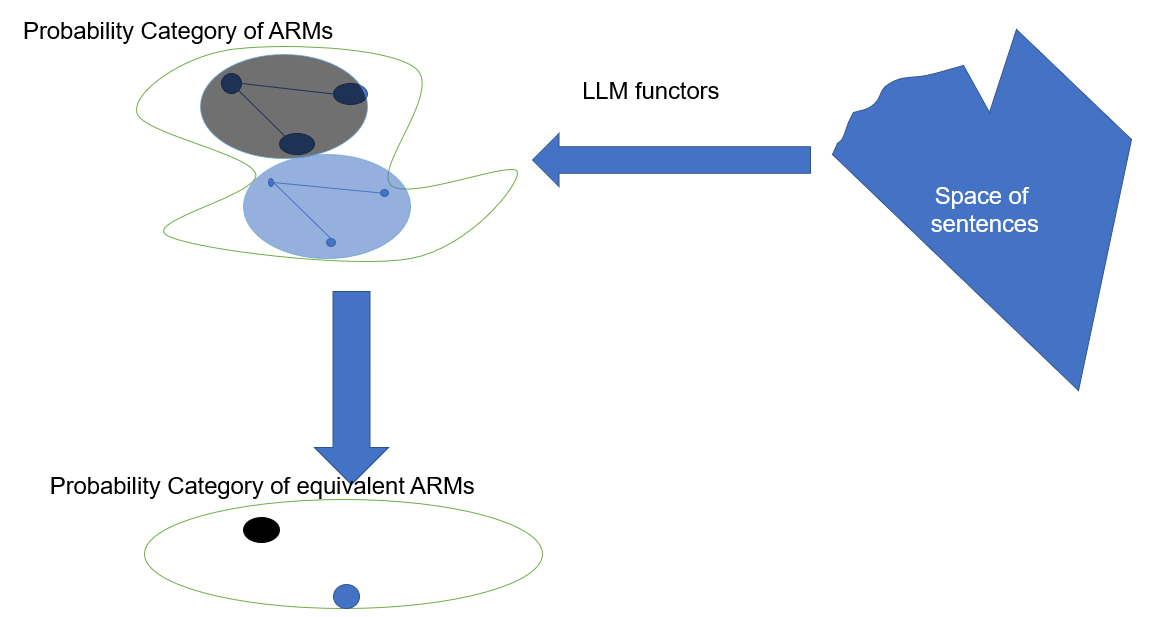
\includegraphics[width=1\linewidth]{Images/GDL/new_AMR_structure.png}
    \caption{Ý tưởng cấu trúc mới về AMR. (LLM functors nghĩa là sử dụng LLM để chuyển một câu sang AMR)}
\end{figure}

Ngoài ra, việc so sánh các đồ thị AMR từ các câu đồng nghĩa cũng mở ra hướng nghiên cứu về các phép biến đổi giữa các đồ thị này. Chúng ta có thể xem xét cách các đồ thị AMR biến đổi khi có sự thay đổi trong cách diễn đạt ngôn ngữ tự nhiên, từ đó xây dựng các mô hình dự đoán hoặc phân loại dựa trên các biến đổi này. Điều này không chỉ giúp hiểu rõ hơn về cấu trúc ngữ nghĩa mà còn có thể ứng dụng trong việc cải thiện các mô hình ngôn ngữ, như mô hình dịch máy hoặc tóm tắt văn bản, bằng cách khai thác sự tương quan giữa các biểu diễn AMR khác nhau trong ngữ cảnh cụ thể.

Sự kết hợp (compose) của các hàm tử (functors) tạo ra các dạng tương đương AMR mới chưa được ghi nhận trong tài liệu hiện có, và những tương đương này có thể được tính toán một cách tự động thông qua mô hình ngôn ngữ lớn (Large Language Model).

Tiếp theo, báo cáo sẽ lấy một ví dụ dịch một câu sang các ngôn ngữ khác nhau rồi dịch trở lại ngon ngữ ban đầu (hình \ref{fig:amr_trans}).

\begin{figure}[H]
    \centering
    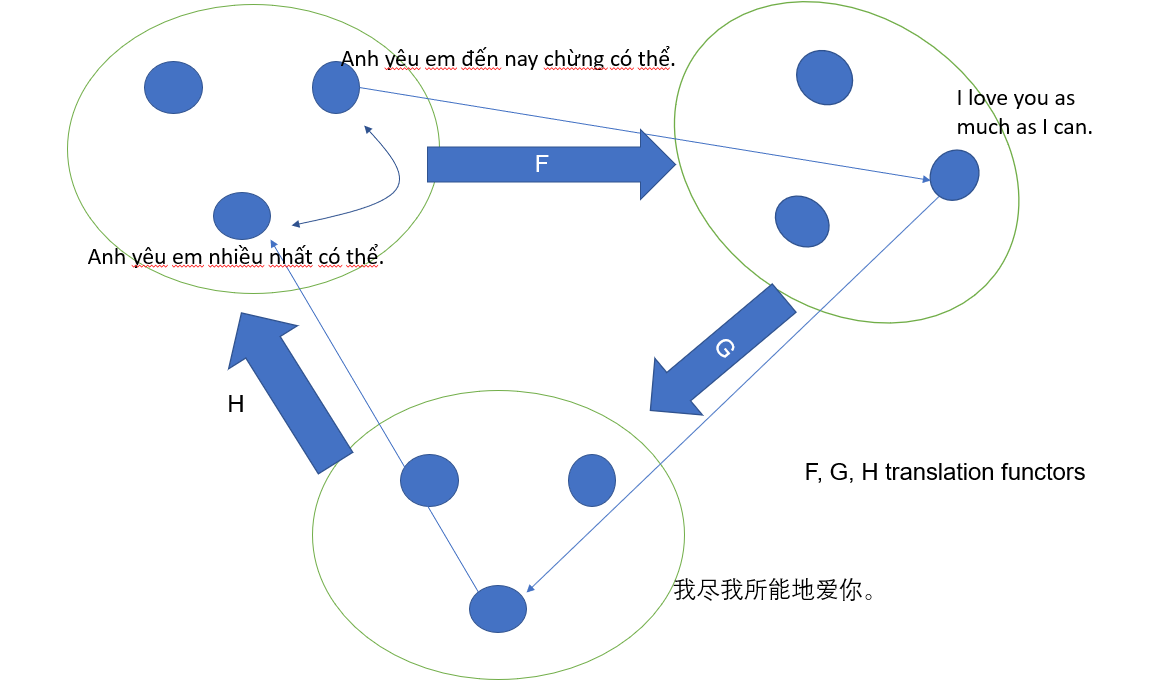
\includegraphics[width=1\linewidth]{Images/GDL/amr_translation.png}
    \caption{Ví dụ minh họa bằng dịch một câu sang ngôn ngữ khác. Những điểm trong hình tròn là các câu khác nhau nhưng cùng nghĩa. F, G, F là các phép dịch một ngôn ngữ này sang ngôn ngữ khác.}
    \label{fig:amr_trans}
\end{figure}
Từ hình \ref{fig:amr_trans} cho thấy trong quá trình dịch và biểu diễn ngữ nghĩa của câu qua nhiều ngôn ngữ. Khi một câu được dịch qua các ngôn ngữ khác nhau (được biểu thị bằng các hàm ánh xạ F, G, H) rồi quay trở lại ngôn ngữ ban đầu, kết quả thu được thường là một câu mới nhưng vẫn giữ nguyên ý nghĩa cốt lõi của câu gốc.

Các hàm ánh xạ F, G, H được coi là các phép biến đổi 1-1 giữa các không gian ngôn ngữ. Tuy nhiên, khi xét đến không gian biểu diễn ngữ nghĩa trừu tượng như AMR (Abstract Meaning Representation), phép nâng (lifting) không còn là phép đồng nhất (identity) mà chỉ còn là phép tương đương (equivalence).

Điều này có nghĩa là các đồ thị AMR của các câu đồng nghĩa, dù có thể khác nhau về cấu trúc cụ thể, nhưng vẫn nên có một mức độ tương đồng nhất định. Ta có thể quantify mức độ tương đồng này bằng một xác suất hay độ đo tương đương nào đó.

Hiện tượng này phản ánh bản chất phức tạp của ngôn ngữ tự nhiên, nơi cùng một ý nghĩa có thể được diễn đạt bằng nhiều cách khác nhau, không chỉ trong cùng một ngôn ngữ mà còn qua các ngôn ngữ khác nhau. Nó cũng cho thấy sự cần thiết của các phương pháp biểu diễn ngữ nghĩa linh hoạt như AMR, có khả năng nắm bắt được bản chất ngữ nghĩa của câu mà không bị ràng buộc quá chặt vào cấu trúc cú pháp cụ thể.

Cuối cùng, nhận xét này gợi ý rằng trong các ứng dụng xử lý ngôn ngữ tự nhiên, đặc biệt là trong lĩnh vực dịch máy và so sánh ngữ nghĩa giữa các câu, ta nên tập trung vào việc phát triển các phương pháp đánh giá độ tương đồng ngữ nghĩa dựa trên các biểu diễn trừu tượng như AMR, thay vì chỉ dựa vào sự giống nhau về mặt từ vựng hay cú pháp.

\begin{figure}[H]
    \centering
    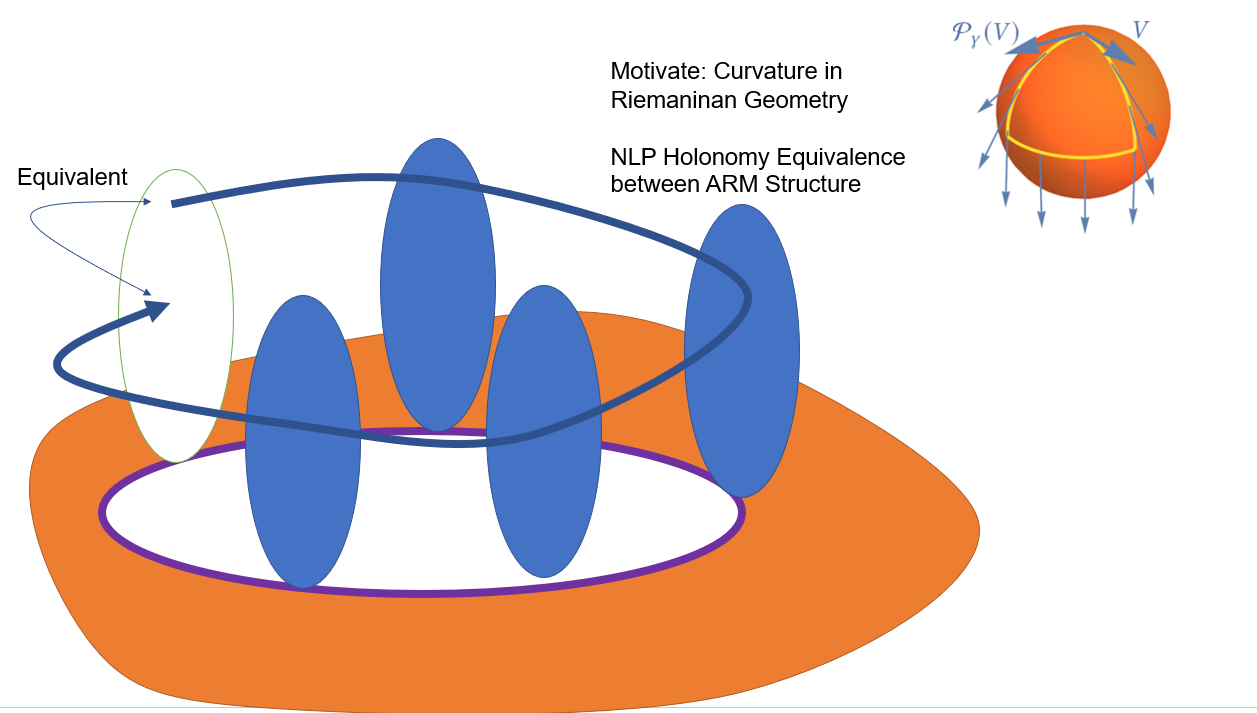
\includegraphics[width=1\linewidth]{Images/GDL/Riemanian_motivation.png}
    \caption{Motivation từ Curvature in Riemaninan Geometry cho cấu trúc AMR trong NLP}
\end{figure}